\section{Topological data analysis, persistent homology}

In this section we introduce a method for analysing a text
without a parameter (e.g.\ k in KNN). In fact, we consider all
the possibilities of parameters. Moreover, we want to be able to
find a meaningful correspondence between the computation and
the text. We use persistent homology.

But for this matter, for simplicity and the reason of capacity
of the author, we have to change our task.

This is a project report instead of a course note, so the importance
is not on the details of the algorithm but rather the ideas and experiments.
But the algorithm and the theory in themselves are interesting and not
easy to be found clearly on the internet, so for the clearness of the report
we include concisely the necessary
concepts and key algorithms there \ref{theoretical}.

\subsection{Essay grading}

Inherently, persistent homology is useful when it comes to 3d modeling.
But in data analysis in general, it is also useful (e.g.\ analyse the
performance of a basketball team and get a intuitive view of the team structure).

Here we use the persistent homology to analyse essays and grading.

Roughly speaking, a better discoursive essay should have a
richer writting structure, (a proposition should be discussed
in different angles, the last paragraph echos to the beginning etc.).
Translated in persistent homology,
if a good essay is a topological space, it should have
many holes (homology groups). For example,
in Figure~\ref{apple}, the essay have a statement, and then some arguments,
, finally a conclusion. 1 - 2 - 3 - 4 are linked by time order, 1 - 4 are linked because they are similar.
This hole means good argument. There are also filled triangles (2-simplices), those
sentences form clusters, so they are filled instead of forming holes.
(We are going to introduce how to build concretely simplicial complexes very soon.)

\begin{figure}[H]
  \centering
  

\tikzset{every picture/.style={line width=0.75pt}} %set default line width to 0.75pt        

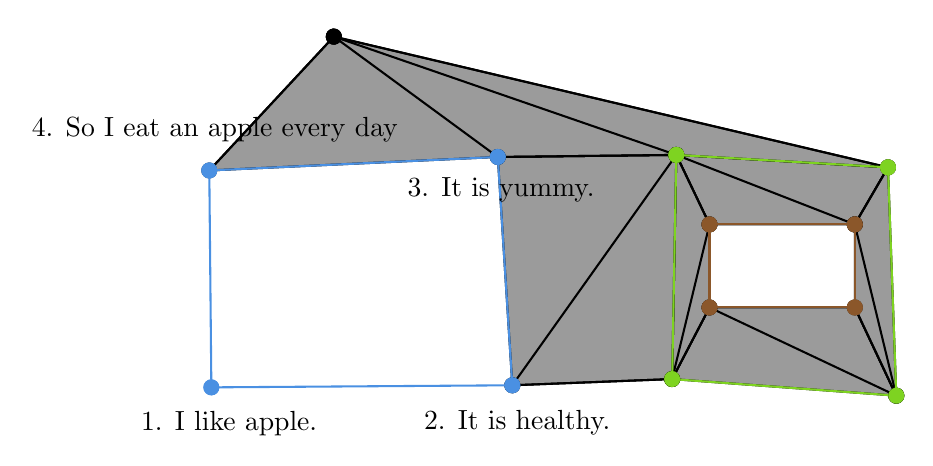
\begin{tikzpicture}[x=0.75pt,y=0.75pt,yscale=-1,xscale=1]
%uncomment if require: \path (0,300); %set diagram left start at 0, and has height of 300

%Shape: Polygon [id:ds506045927728886] 
\draw  [fill={rgb, 255:red, 155; green, 155; blue, 155 }  ,fill opacity=1 ] (337,211.5) -- (355,177) -- (425,177) -- (445,219.5) -- cycle ;
%Shape: Polygon [id:ds373063136182463] 
\draw  [fill={rgb, 255:red, 155; green, 155; blue, 155 }  ,fill opacity=1 ] (441,109.5) -- (425,137) -- (355,137) -- (339,103.5) -- cycle ;
%Shape: Polygon [id:ds04357467087348055] 
\draw  [fill={rgb, 255:red, 155; green, 155; blue, 155 }  ,fill opacity=1 ] (445,219.5) -- (425,177) -- (425,137) -- (441,109.5) -- cycle ;
%Shape: Polygon [id:ds8597694080078087] 
\draw  [fill={rgb, 255:red, 155; green, 155; blue, 155 }  ,fill opacity=1 ] (339,103.5) -- (355,137) -- (355,177) -- (337,211.5) -- cycle ;

%Straight Lines [id:da7958699538877538] 
\draw    (339,103.5) -- (425,137) ;
\draw [shift={(425,137)}, rotate = 21.28] [color={rgb, 255:red, 0; green, 0; blue, 0 }  ][fill={rgb, 255:red, 0; green, 0; blue, 0 }  ][line width=0.75]      (0, 0) circle [x radius= 3.35, y radius= 3.35]   ;
\draw [shift={(339,103.5)}, rotate = 21.28] [color={rgb, 255:red, 0; green, 0; blue, 0 }  ][fill={rgb, 255:red, 0; green, 0; blue, 0 }  ][line width=0.75]      (0, 0) circle [x radius= 3.35, y radius= 3.35]   ;
%Straight Lines [id:da37382810612047734] 
\draw    (425,137) -- (445,219.5) ;
\draw [shift={(445,219.5)}, rotate = 76.37] [color={rgb, 255:red, 0; green, 0; blue, 0 }  ][fill={rgb, 255:red, 0; green, 0; blue, 0 }  ][line width=0.75]      (0, 0) circle [x radius= 3.35, y radius= 3.35]   ;
\draw [shift={(425,137)}, rotate = 76.37] [color={rgb, 255:red, 0; green, 0; blue, 0 }  ][fill={rgb, 255:red, 0; green, 0; blue, 0 }  ][line width=0.75]      (0, 0) circle [x radius= 3.35, y radius= 3.35]   ;
%Straight Lines [id:da33578118329024775] 
\draw    (355,177) -- (445,219.5) ;
\draw [shift={(445,219.5)}, rotate = 25.28] [color={rgb, 255:red, 0; green, 0; blue, 0 }  ][fill={rgb, 255:red, 0; green, 0; blue, 0 }  ][line width=0.75]      (0, 0) circle [x radius= 3.35, y radius= 3.35]   ;
\draw [shift={(355,177)}, rotate = 25.28] [color={rgb, 255:red, 0; green, 0; blue, 0 }  ][fill={rgb, 255:red, 0; green, 0; blue, 0 }  ][line width=0.75]      (0, 0) circle [x radius= 3.35, y radius= 3.35]   ;
%Straight Lines [id:da27555178758587107] 
\draw    (355,137) -- (337,211.5) ;
\draw [shift={(337,211.5)}, rotate = 103.58] [color={rgb, 255:red, 0; green, 0; blue, 0 }  ][fill={rgb, 255:red, 0; green, 0; blue, 0 }  ][line width=0.75]      (0, 0) circle [x radius= 3.35, y radius= 3.35]   ;
\draw [shift={(355,137)}, rotate = 103.58] [color={rgb, 255:red, 0; green, 0; blue, 0 }  ][fill={rgb, 255:red, 0; green, 0; blue, 0 }  ][line width=0.75]      (0, 0) circle [x radius= 3.35, y radius= 3.35]   ;
%Shape: Polygon [id:ds20124875657376728] 
\draw  [fill={rgb, 255:red, 155; green, 155; blue, 155 }  ,fill opacity=1 ] (253,104.5) -- (260,214.5) -- (337,211.5) -- (339,103.5) -- cycle ;
%Shape: Polygon [id:ds3619467537546437] 
\draw  [fill={rgb, 255:red, 155; green, 155; blue, 155 }  ,fill opacity=1 ] (174,46.5) -- (441,109.5) -- (339,103.5) -- (253,104.5) -- (114,111) -- cycle ;
%Straight Lines [id:da5963075508320128] 
\draw    (339,103.5) -- (253,104.5) ;
\draw [shift={(253,104.5)}, rotate = 179.33] [color={rgb, 255:red, 0; green, 0; blue, 0 }  ][fill={rgb, 255:red, 0; green, 0; blue, 0 }  ][line width=0.75]      (0, 0) circle [x radius= 3.35, y radius= 3.35]   ;
\draw [shift={(339,103.5)}, rotate = 179.33] [color={rgb, 255:red, 0; green, 0; blue, 0 }  ][fill={rgb, 255:red, 0; green, 0; blue, 0 }  ][line width=0.75]      (0, 0) circle [x radius= 3.35, y radius= 3.35]   ;
%Straight Lines [id:da8612090103920278] 
\draw    (260,214.5) -- (339,103.5) ;
\draw [shift={(339,103.5)}, rotate = 305.44] [color={rgb, 255:red, 0; green, 0; blue, 0 }  ][fill={rgb, 255:red, 0; green, 0; blue, 0 }  ][line width=0.75]      (0, 0) circle [x radius= 3.35, y radius= 3.35]   ;
\draw [shift={(260,214.5)}, rotate = 305.44] [color={rgb, 255:red, 0; green, 0; blue, 0 }  ][fill={rgb, 255:red, 0; green, 0; blue, 0 }  ][line width=0.75]      (0, 0) circle [x radius= 3.35, y radius= 3.35]   ;
%Straight Lines [id:da9692653745827828] 
\draw    (260,214.5) -- (337,211.5) ;
\draw [shift={(337,211.5)}, rotate = 357.77] [color={rgb, 255:red, 0; green, 0; blue, 0 }  ][fill={rgb, 255:red, 0; green, 0; blue, 0 }  ][line width=0.75]      (0, 0) circle [x radius= 3.35, y radius= 3.35]   ;
\draw [shift={(260,214.5)}, rotate = 357.77] [color={rgb, 255:red, 0; green, 0; blue, 0 }  ][fill={rgb, 255:red, 0; green, 0; blue, 0 }  ][line width=0.75]      (0, 0) circle [x radius= 3.35, y radius= 3.35]   ;
%Straight Lines [id:da7164877740446134] 
\draw    (114,111) -- (174,46.5) ;
\draw [shift={(174,46.5)}, rotate = 312.93] [color={rgb, 255:red, 0; green, 0; blue, 0 }  ][fill={rgb, 255:red, 0; green, 0; blue, 0 }  ][line width=0.75]      (0, 0) circle [x radius= 3.35, y radius= 3.35]   ;
\draw [shift={(114,111)}, rotate = 312.93] [color={rgb, 255:red, 0; green, 0; blue, 0 }  ][fill={rgb, 255:red, 0; green, 0; blue, 0 }  ][line width=0.75]      (0, 0) circle [x radius= 3.35, y radius= 3.35]   ;
%Straight Lines [id:da2125405974487078] 
\draw    (174,46.5) -- (253,104.5) ;
\draw [shift={(253,104.5)}, rotate = 36.29] [color={rgb, 255:red, 0; green, 0; blue, 0 }  ][fill={rgb, 255:red, 0; green, 0; blue, 0 }  ][line width=0.75]      (0, 0) circle [x radius= 3.35, y radius= 3.35]   ;
\draw [shift={(174,46.5)}, rotate = 36.29] [color={rgb, 255:red, 0; green, 0; blue, 0 }  ][fill={rgb, 255:red, 0; green, 0; blue, 0 }  ][line width=0.75]      (0, 0) circle [x radius= 3.35, y radius= 3.35]   ;
%Straight Lines [id:da8884288301278187] 
\draw    (174,46.5) -- (441,109.5) ;
\draw [shift={(441,109.5)}, rotate = 13.28] [color={rgb, 255:red, 0; green, 0; blue, 0 }  ][fill={rgb, 255:red, 0; green, 0; blue, 0 }  ][line width=0.75]      (0, 0) circle [x radius= 3.35, y radius= 3.35]   ;
\draw [shift={(174,46.5)}, rotate = 13.28] [color={rgb, 255:red, 0; green, 0; blue, 0 }  ][fill={rgb, 255:red, 0; green, 0; blue, 0 }  ][line width=0.75]      (0, 0) circle [x radius= 3.35, y radius= 3.35]   ;
%Straight Lines [id:da3878057357434834] 
\draw    (174,46.5) -- (339,103.5) ;
\draw [shift={(339,103.5)}, rotate = 19.06] [color={rgb, 255:red, 0; green, 0; blue, 0 }  ][fill={rgb, 255:red, 0; green, 0; blue, 0 }  ][line width=0.75]      (0, 0) circle [x radius= 3.35, y radius= 3.35]   ;
\draw [shift={(174,46.5)}, rotate = 19.06] [color={rgb, 255:red, 0; green, 0; blue, 0 }  ][fill={rgb, 255:red, 0; green, 0; blue, 0 }  ][line width=0.75]      (0, 0) circle [x radius= 3.35, y radius= 3.35]   ;
%Straight Lines [id:da3895078416872] 
\draw [color={rgb, 255:red, 126; green, 211; blue, 33 }  ,draw opacity=1 ]   (445,219.5) -- (337,211.5) ;
\draw [shift={(337,211.5)}, rotate = 184.24] [color={rgb, 255:red, 126; green, 211; blue, 33 }  ,draw opacity=1 ][fill={rgb, 255:red, 126; green, 211; blue, 33 }  ,fill opacity=1 ][line width=0.75]      (0, 0) circle [x radius= 3.35, y radius= 3.35]   ;
\draw [shift={(445,219.5)}, rotate = 184.24] [color={rgb, 255:red, 126; green, 211; blue, 33 }  ,draw opacity=1 ][fill={rgb, 255:red, 126; green, 211; blue, 33 }  ,fill opacity=1 ][line width=0.75]      (0, 0) circle [x radius= 3.35, y radius= 3.35]   ;
%Straight Lines [id:da300892222460144] 
\draw [color={rgb, 255:red, 74; green, 144; blue, 226 }  ,draw opacity=1 ]   (114,111) -- (115,215.5) ;
\draw [shift={(115,215.5)}, rotate = 89.45] [color={rgb, 255:red, 74; green, 144; blue, 226 }  ,draw opacity=1 ][fill={rgb, 255:red, 74; green, 144; blue, 226 }  ,fill opacity=1 ][line width=0.75]      (0, 0) circle [x radius= 3.35, y radius= 3.35]   ;
\draw [shift={(114,111)}, rotate = 89.45] [color={rgb, 255:red, 74; green, 144; blue, 226 }  ,draw opacity=1 ][fill={rgb, 255:red, 74; green, 144; blue, 226 }  ,fill opacity=1 ][line width=0.75]      (0, 0) circle [x radius= 3.35, y radius= 3.35]   ;
%Straight Lines [id:da5712067967796253] 
\draw [color={rgb, 255:red, 74; green, 144; blue, 226 }  ,draw opacity=1 ]   (115,215.5) -- (260,214.5) ;
\draw [shift={(260,214.5)}, rotate = 359.6] [color={rgb, 255:red, 74; green, 144; blue, 226 }  ,draw opacity=1 ][fill={rgb, 255:red, 74; green, 144; blue, 226 }  ,fill opacity=1 ][line width=0.75]      (0, 0) circle [x radius= 3.35, y radius= 3.35]   ;
\draw [shift={(115,215.5)}, rotate = 359.6] [color={rgb, 255:red, 74; green, 144; blue, 226 }  ,draw opacity=1 ][fill={rgb, 255:red, 74; green, 144; blue, 226 }  ,fill opacity=1 ][line width=0.75]      (0, 0) circle [x radius= 3.35, y radius= 3.35]   ;
%Straight Lines [id:da998130260097339] 
\draw [color={rgb, 255:red, 74; green, 144; blue, 226 }  ,draw opacity=1 ]   (260,214.5) -- (253,104.5) ;
\draw [shift={(253,104.5)}, rotate = 266.36] [color={rgb, 255:red, 74; green, 144; blue, 226 }  ,draw opacity=1 ][fill={rgb, 255:red, 74; green, 144; blue, 226 }  ,fill opacity=1 ][line width=0.75]      (0, 0) circle [x radius= 3.35, y radius= 3.35]   ;
\draw [shift={(260,214.5)}, rotate = 266.36] [color={rgb, 255:red, 74; green, 144; blue, 226 }  ,draw opacity=1 ][fill={rgb, 255:red, 74; green, 144; blue, 226 }  ,fill opacity=1 ][line width=0.75]      (0, 0) circle [x radius= 3.35, y radius= 3.35]   ;
%Straight Lines [id:da15833915226992357] 
\draw [color={rgb, 255:red, 74; green, 144; blue, 226 }  ,draw opacity=1 ]   (114,111) -- (253,104.5) ;
\draw [shift={(253,104.5)}, rotate = 357.32] [color={rgb, 255:red, 74; green, 144; blue, 226 }  ,draw opacity=1 ][fill={rgb, 255:red, 74; green, 144; blue, 226 }  ,fill opacity=1 ][line width=0.75]      (0, 0) circle [x radius= 3.35, y radius= 3.35]   ;
\draw [shift={(114,111)}, rotate = 357.32] [color={rgb, 255:red, 74; green, 144; blue, 226 }  ,draw opacity=1 ][fill={rgb, 255:red, 74; green, 144; blue, 226 }  ,fill opacity=1 ][line width=0.75]      (0, 0) circle [x radius= 3.35, y radius= 3.35]   ;
%Straight Lines [id:da1551244874188762] 
\draw    (441,109.5) -- (425,137) ;
\draw [shift={(425,137)}, rotate = 120.19] [color={rgb, 255:red, 0; green, 0; blue, 0 }  ][fill={rgb, 255:red, 0; green, 0; blue, 0 }  ][line width=0.75]      (0, 0) circle [x radius= 3.35, y radius= 3.35]   ;
\draw [shift={(441,109.5)}, rotate = 120.19] [color={rgb, 255:red, 0; green, 0; blue, 0 }  ][fill={rgb, 255:red, 0; green, 0; blue, 0 }  ][line width=0.75]      (0, 0) circle [x radius= 3.35, y radius= 3.35]   ;
%Straight Lines [id:da45803051915893067] 
\draw    (425,177) -- (445,219.5) ;
\draw [shift={(445,219.5)}, rotate = 64.8] [color={rgb, 255:red, 0; green, 0; blue, 0 }  ][fill={rgb, 255:red, 0; green, 0; blue, 0 }  ][line width=0.75]      (0, 0) circle [x radius= 3.35, y radius= 3.35]   ;
\draw [shift={(425,177)}, rotate = 64.8] [color={rgb, 255:red, 0; green, 0; blue, 0 }  ][fill={rgb, 255:red, 0; green, 0; blue, 0 }  ][line width=0.75]      (0, 0) circle [x radius= 3.35, y radius= 3.35]   ;
%Straight Lines [id:da3656558768012268] 
\draw    (355,177) -- (337,211.5) ;
\draw [shift={(337,211.5)}, rotate = 117.55] [color={rgb, 255:red, 0; green, 0; blue, 0 }  ][fill={rgb, 255:red, 0; green, 0; blue, 0 }  ][line width=0.75]      (0, 0) circle [x radius= 3.35, y radius= 3.35]   ;
\draw [shift={(355,177)}, rotate = 117.55] [color={rgb, 255:red, 0; green, 0; blue, 0 }  ][fill={rgb, 255:red, 0; green, 0; blue, 0 }  ][line width=0.75]      (0, 0) circle [x radius= 3.35, y radius= 3.35]   ;
%Straight Lines [id:da6696032151723832] 
\draw    (355,137) -- (339,103.5) ;
\draw [shift={(339,103.5)}, rotate = 244.47] [color={rgb, 255:red, 0; green, 0; blue, 0 }  ][fill={rgb, 255:red, 0; green, 0; blue, 0 }  ][line width=0.75]      (0, 0) circle [x radius= 3.35, y radius= 3.35]   ;
\draw [shift={(355,137)}, rotate = 244.47] [color={rgb, 255:red, 0; green, 0; blue, 0 }  ][fill={rgb, 255:red, 0; green, 0; blue, 0 }  ][line width=0.75]      (0, 0) circle [x radius= 3.35, y radius= 3.35]   ;
%Straight Lines [id:da9412473128467516] 
\draw [color={rgb, 255:red, 126; green, 211; blue, 33 }  ,draw opacity=1 ]   (337,211.5) -- (339,103.5) ;
\draw [shift={(339,103.5)}, rotate = 271.06] [color={rgb, 255:red, 126; green, 211; blue, 33 }  ,draw opacity=1 ][fill={rgb, 255:red, 126; green, 211; blue, 33 }  ,fill opacity=1 ][line width=0.75]      (0, 0) circle [x radius= 3.35, y radius= 3.35]   ;
\draw [shift={(337,211.5)}, rotate = 271.06] [color={rgb, 255:red, 126; green, 211; blue, 33 }  ,draw opacity=1 ][fill={rgb, 255:red, 126; green, 211; blue, 33 }  ,fill opacity=1 ][line width=0.75]      (0, 0) circle [x radius= 3.35, y radius= 3.35]   ;
%Straight Lines [id:da40626776597378655] 
\draw [color={rgb, 255:red, 126; green, 211; blue, 33 }  ,draw opacity=1 ]   (441,109.5) -- (445,219.5) ;
\draw [shift={(445,219.5)}, rotate = 87.92] [color={rgb, 255:red, 126; green, 211; blue, 33 }  ,draw opacity=1 ][fill={rgb, 255:red, 126; green, 211; blue, 33 }  ,fill opacity=1 ][line width=0.75]      (0, 0) circle [x radius= 3.35, y radius= 3.35]   ;
\draw [shift={(441,109.5)}, rotate = 87.92] [color={rgb, 255:red, 126; green, 211; blue, 33 }  ,draw opacity=1 ][fill={rgb, 255:red, 126; green, 211; blue, 33 }  ,fill opacity=1 ][line width=0.75]      (0, 0) circle [x radius= 3.35, y radius= 3.35]   ;
%Straight Lines [id:da39887955488152826] 
\draw [color={rgb, 255:red, 126; green, 211; blue, 33 }  ,draw opacity=1 ]   (441,109.5) -- (339,103.5) ;
\draw [shift={(339,103.5)}, rotate = 183.37] [color={rgb, 255:red, 126; green, 211; blue, 33 }  ,draw opacity=1 ][fill={rgb, 255:red, 126; green, 211; blue, 33 }  ,fill opacity=1 ][line width=0.75]      (0, 0) circle [x radius= 3.35, y radius= 3.35]   ;
\draw [shift={(441,109.5)}, rotate = 183.37] [color={rgb, 255:red, 126; green, 211; blue, 33 }  ,draw opacity=1 ][fill={rgb, 255:red, 126; green, 211; blue, 33 }  ,fill opacity=1 ][line width=0.75]      (0, 0) circle [x radius= 3.35, y radius= 3.35]   ;
%Straight Lines [id:da42956969917858223] 
\draw [color={rgb, 255:red, 139; green, 87; blue, 42 }  ,draw opacity=1 ]   (425,137) -- (355,137) ;
\draw [shift={(355,137)}, rotate = 180] [color={rgb, 255:red, 139; green, 87; blue, 42 }  ,draw opacity=1 ][fill={rgb, 255:red, 139; green, 87; blue, 42 }  ,fill opacity=1 ][line width=0.75]      (0, 0) circle [x radius= 3.35, y radius= 3.35]   ;
\draw [shift={(425,137)}, rotate = 180] [color={rgb, 255:red, 139; green, 87; blue, 42 }  ,draw opacity=1 ][fill={rgb, 255:red, 139; green, 87; blue, 42 }  ,fill opacity=1 ][line width=0.75]      (0, 0) circle [x radius= 3.35, y radius= 3.35]   ;
%Straight Lines [id:da14852397184426325] 
\draw [color={rgb, 255:red, 139; green, 87; blue, 42 }  ,draw opacity=1 ]   (425,177) -- (425,137) ;
\draw [shift={(425,137)}, rotate = 270] [color={rgb, 255:red, 139; green, 87; blue, 42 }  ,draw opacity=1 ][fill={rgb, 255:red, 139; green, 87; blue, 42 }  ,fill opacity=1 ][line width=0.75]      (0, 0) circle [x radius= 3.35, y radius= 3.35]   ;
\draw [shift={(425,177)}, rotate = 270] [color={rgb, 255:red, 139; green, 87; blue, 42 }  ,draw opacity=1 ][fill={rgb, 255:red, 139; green, 87; blue, 42 }  ,fill opacity=1 ][line width=0.75]      (0, 0) circle [x radius= 3.35, y radius= 3.35]   ;
%Straight Lines [id:da7173822720349425] 
\draw [color={rgb, 255:red, 139; green, 87; blue, 42 }  ,draw opacity=1 ]   (355,177) -- (425,177) ;
\draw [shift={(425,177)}, rotate = 0] [color={rgb, 255:red, 139; green, 87; blue, 42 }  ,draw opacity=1 ][fill={rgb, 255:red, 139; green, 87; blue, 42 }  ,fill opacity=1 ][line width=0.75]      (0, 0) circle [x radius= 3.35, y radius= 3.35]   ;
\draw [shift={(355,177)}, rotate = 0] [color={rgb, 255:red, 139; green, 87; blue, 42 }  ,draw opacity=1 ][fill={rgb, 255:red, 139; green, 87; blue, 42 }  ,fill opacity=1 ][line width=0.75]      (0, 0) circle [x radius= 3.35, y radius= 3.35]   ;
%Straight Lines [id:da6148683084406998] 
\draw [color={rgb, 255:red, 139; green, 87; blue, 42 }  ,draw opacity=1 ]   (355,177) -- (355,137) ;
\draw [shift={(355,137)}, rotate = 270] [color={rgb, 255:red, 139; green, 87; blue, 42 }  ,draw opacity=1 ][fill={rgb, 255:red, 139; green, 87; blue, 42 }  ,fill opacity=1 ][line width=0.75]      (0, 0) circle [x radius= 3.35, y radius= 3.35]   ;
\draw [shift={(355,177)}, rotate = 270] [color={rgb, 255:red, 139; green, 87; blue, 42 }  ,draw opacity=1 ][fill={rgb, 255:red, 139; green, 87; blue, 42 }  ,fill opacity=1 ][line width=0.75]      (0, 0) circle [x radius= 3.35, y radius= 3.35]   ;

% Text Node
\draw (79.67,225.67) node [anchor=north west][inner sep=0.75pt]   [align=left] {1. I like apple.};
% Text Node
\draw (216,225) node [anchor=north west][inner sep=0.75pt]   [align=left] {2. It is healthy.};
% Text Node
\draw (208,113) node [anchor=north west][inner sep=0.75pt]   [align=left] {3. It is yummy.};
% Text Node
\draw (27,84) node [anchor=north west][inner sep=0.75pt]   [align=left] {4. So I eat an apple every day};


\end{tikzpicture}
  \caption{There are 2 holes in this simplicial complex,
  one represented by the blue cycle and one by brown.
  Note that the brown cycle and the green cycle are homology equivalent, so they count as one.}
  \label{apple}
\end{figure}

If we only have one such graph, we will have to determine the similarity to link.
However, different similarity bars can give different simplicial complexes and have
different homology groups. Structure changes with scale, e.g.\ Figure~\ref{fig:scale}.
So our approache will consider all the scales (whence ``persistent'' homology).

\begin{figure}[H]
\centering
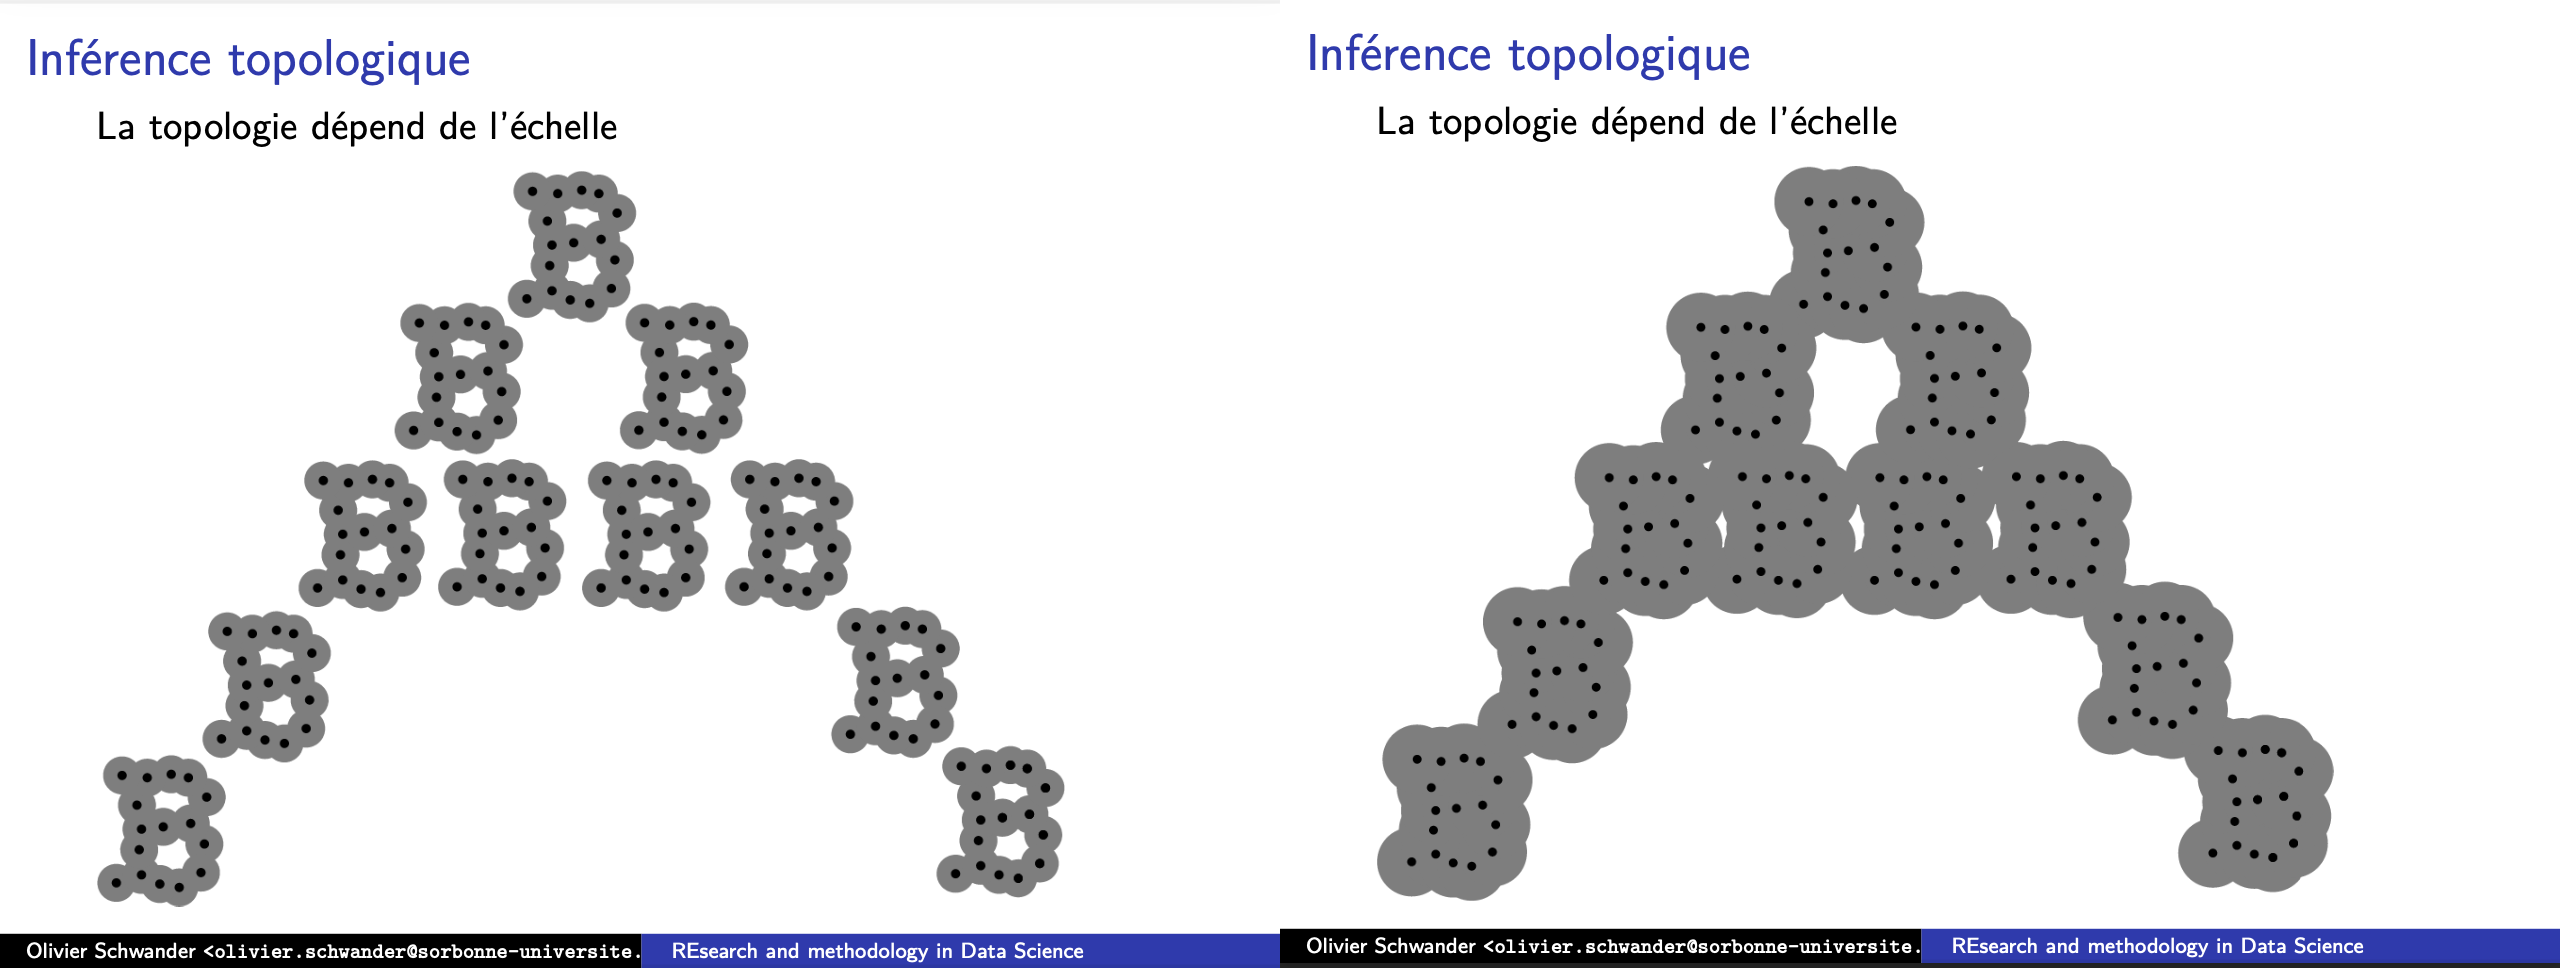
\includegraphics[width=14cm]{scale.png}
\caption{Structure changes with scale}
\label{fig:scale}
\end{figure}

\begin{figure}[H]
  \centering
  \begin{tikzpicture}[scale=0.4]

  \coordinate (v1) at (0,0);
  \coordinate (v2) at (0,3);
  \coordinate (v3) at (3,0);
  \coordinate (v4) at (3,3);
  \draw (v1) -- (v2);
  \draw (v3) -- (v4);
  \draw (v1) -- (v3);

  \coordinate (w1) at (8+0,0);
  \coordinate (w2) at (8+0,3);
  \coordinate (w3) at (8+3,0);
  \coordinate (w4) at (8+3,3);
  \draw (w1) -- (w2);
  \draw (w3) -- (w4);
  \draw (w1) -- (w3);
  \draw (w2) -- (w4);
  \draw[->] (4,1.5) -- (7,1.5);

  \coordinate (u1) at (16+0,0);
  \coordinate (u2) at (16+0,3);
  \coordinate (u3) at (16+3,0);
  \coordinate (u4) at (16+3,3);
  \draw (u1) -- (u2);
  \draw (u3) -- (u4);
  \draw (u1) -- (u3);
  \draw (u2) -- (u4);
  \draw (u1) -- (u4);
  \draw[->] (12,1.5) -- (15,1.5);

  \coordinate (uu1) at (24+0,0);
  \coordinate (uu2) at (24+0,3);
  \coordinate (uu3) at (24+3,0);
  \coordinate (uu4) at (24+3,3);
  \draw (uu1) -- (uu2);
  \draw (uu3) -- (uu4);
  \draw (uu1) -- (uu3);
  \draw (uu2) -- (uu4);
  \draw (uu1) -- (uu4);
  \filldraw[fill=gray] (uu1) -- (uu4) -- (uu2);
  \draw[->] (20,1.5) -- (23,1.5);

  \foreach \vertex in {v1,v2,v3,v4,w1,w2,w3,w4,
  u1,u2,u3,u4,
  uu1,uu2,uu3,uu4}
    \fill (\vertex) circle (5pt);

  \coordinate (d) at (1.5,-0.5);
  \draw[->] ($(v1)+(d)$) -- node[left] {$H_1$} ++(0,-2) node[below] {$\K^0$};
  \draw[->] ($(w1)+(d)$) -- ++(0,-2) node[below] {$\K^1$};
  \draw[->] ($(u1)+(d)$) -- ++(0,-2) node[below] {$\K^2$};
  \draw[->] ($(uu1)+(d)$) -- ++(0,-2) node[below] {$\K^1$};

  \draw[->] (4, -2.75) -- node[above] {$0$}++(3,0);
  \draw[->] (12,-2.75) -- node[above] {$\begin{pmatrix}1\\0 \end{pmatrix}$}++(3,0);
  \draw[->] (20,-2.75) -- node[above] {$\begin{pmatrix}1 & 0 \end{pmatrix}$}++(3,0);
  
  \node at (13.5,-4.5) {\rotatebox{270}{$\simeq$}};
  \node at (13.5,-6) {$\I_{[2, \infty)} \oplus \I_{[3, 4)}$};

\end{tikzpicture}
  \caption{Filtration gives persistence module gives decomposition gives barcodes}
  \label{fig:tda_diagram}
  \end{figure}

\paragraph{Similarity Filtration with Time Skeleton (SIFTS) \cite{Zhu_2013}}

As in KNN we choose an embedding and a
distance. Then we construct a filtration (a sequence of inclusions
of simplical complexes) of Rips Complexes.

\begin{definition}[Rips complex]
  Given a symmetric matrix $M \in M_n(R^+)$, we define a filtration of Rips complexes
  $$
  (V_d := \{A \subset \llbracket 1, n\rrbracket :
  \forall 1\le i<j\le n, M_{i, j} \le d\})_{d\ge 0}
  $$
\end{definition}
\RM A simplex appears when the last appearance of the its faces happens.

Given an essay, we split it to sentences in order. We embed each sentence by tf-idf.
Then we construct our matrix $M$ by setting $M_{i, j} = 1-\cos(\theta_{i,j})~\text{(the cosine distance)}$
where $\theta_{i, j}$ is the angle between the vectors embedded by the ith and jth sentences.
Then we set $M_{i, i+1} = 0$ (this is where the ``time skeleton'' come from, the reason is
to preserve the order of the essay). We obtain then
a filtration of Rips complexes.
In the filtration, what all this means is that,
at index 0, we will have a skeleton from the first sentence to the last sentence,
then we add simplexes with closer points then those with further points.

After having the filtration, we count the ``number of holes'' of dimension 1
that appears in the filtration (this is formally the \textbf{number of
barcodes} of dimension 1 after we decompose the persistence module
induced by the filtration c.f.\ Figure~\ref{fig:tda_diagram}).
Note that if we just count the number of holes at each index for the filtration,
it would be trivial and not useful, we have to be able to identity the holes
throughout the filtration so that we don't count a hole twice.

We hope to show that this number of holes reflects the quality of arguments of an essay.

\paragraph{Experiment on a real set of data}

data source (more precisely, the essay set 2, which is discoursive) :
\url{https://www.kaggle.com/datasets/thevirusx3/automated-essay-scoring-dataset/code?select=training_set_rel3.tsv}

\begin{figure}[H]
\begin{minipage}{0.49\linewidth}
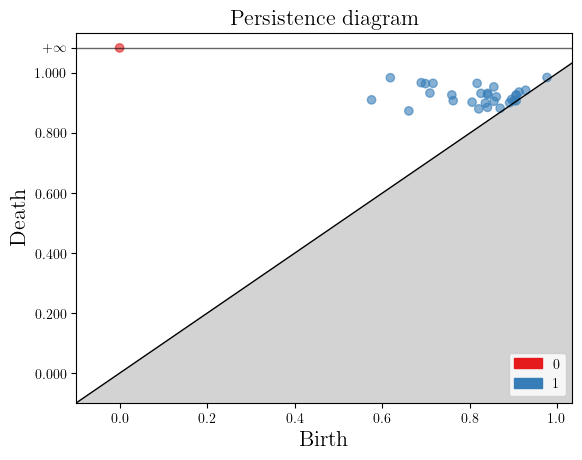
\includegraphics[width=8cm]{pdessay.png}
\end{minipage}
\begin{minipage}{0.49\linewidth}
In @DATE1's world, there are many things found offensive.  Everyone has their own opinion on what is offensive and what is not. Many parents are becoming upset because they think their children are viewing things that they should not.  Other people are upset because they think the libraries are offending their culture or way of life.  This is even taken to the extreme where people want censhorship on libraries to avoid this, which is wrong.     Some people are becoming concerned about the materials in libraries.  They find these things to be offensive.  Everyone is entitled to their own opinion, but there really is nothing anyone can do if someone is offended.  The world is a public place and everywhere we go, something might be found offensive.  The library is a place for study.  It is never intended to offend someone, or bring bad to the world.  It is simply a place to inform, and if someone is offended by what they see, they should stay away from the library.     I have been to the library many times, none of which have I ever seen anything offensive.  Everything I have ever witnessed at the library is for learning and research...
\end{minipage}
\caption{The persistence diagram of an essay of grade 4/6 : A point $(x, y)$ in this diagram corresponds to
a interval module of extremities $x, y$ in the homology of certain degree.
We have many blue points meaning many holes in dim 1, one red point meaning
one homology group of dim 1
}
\label{fig:pd}
\end{figure}

\begin{figure}[H]
% \centering
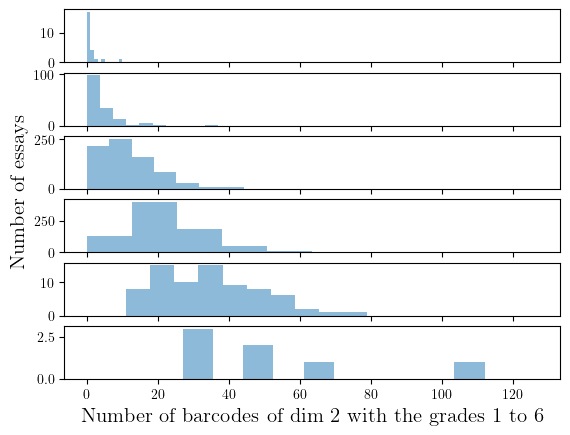
\includegraphics[width=8cm]{gradesh1.png}
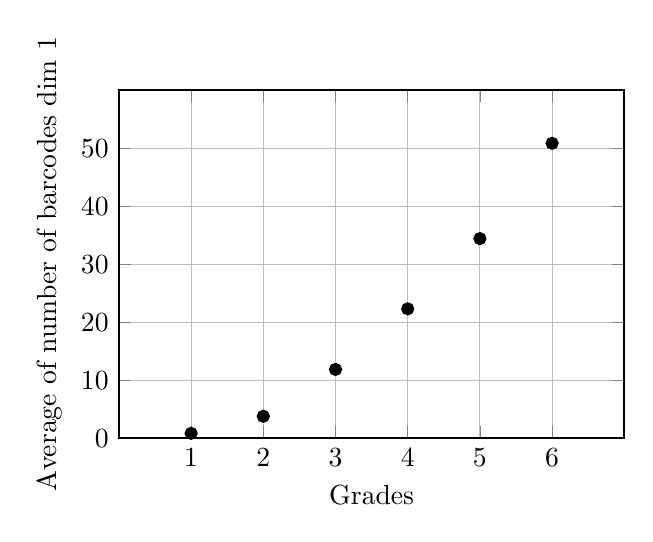
\begin{tikzpicture}
  \begin{axis}[
    xlabel={Grades},
    ylabel={Average of number of barcodes dim 1},
    grid=both,
    xmin=0,
    ymin=0,
    xmax=7,
    ymax=60,
    xtick={1,2,3,4,5,6},
    ytick={0,10,20,30,40,50},
    width=8cm,
    height=6cm,
    ]
    
    \addplot[only marks, mark=*, mark size=2pt] coordinates {
        (1, 0.8333333333333334)
        (2, 3.7777777777777777)
        (3, 11.857142857142858)
        (4, 22.308483290488432)
        (5, 34.42666666666667)
        (6, 50.857142857142854)
    };
  \end{axis}
\end{tikzpicture}
\caption{Number of barcodes increases as grade increases}
\label{fig:ds}
\end{figure}

Those are some discoursive essays on the topic of offense/censorship. We first inspect
an essay with grade 4/6 as an example Figure~\ref{fig:pd}. Then we show
the average of number of holes for each grade (1-6)
as well as the average of number of barcodes for each grade (Figure~\ref{fig:ds}).
We find that number of holes increases as grade increases.

But there are other factors other than the richness of structure of the essay that may affect
the number of holes, like the number of sentences (if we have more points in the set
we will have more chances to form holes) or the number of words.

\begin{figure}[H]
  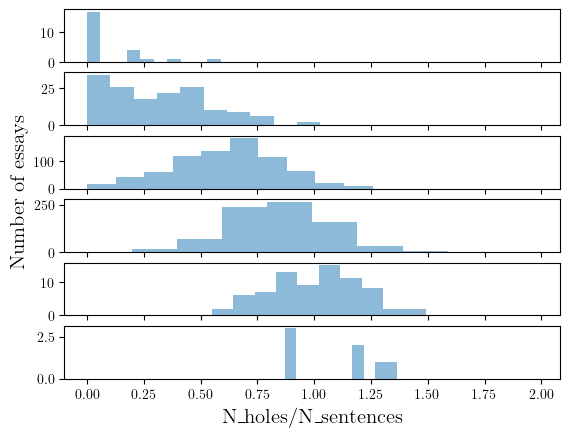
\includegraphics[width=8cm]{gradesah1s.png}
  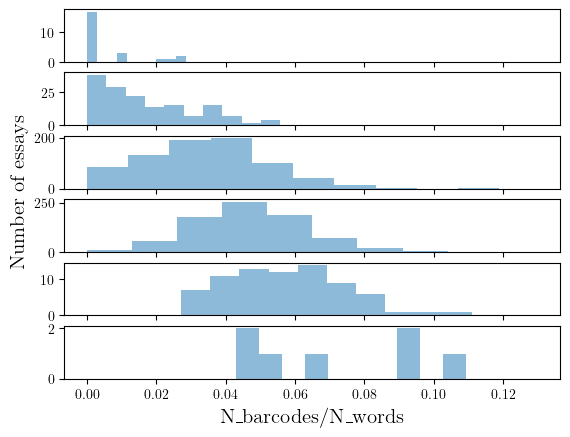
\includegraphics[width=8cm]{gradesah1w.png}
  \caption{The average of barcodes each sentence/word increases as grade increases}
  \label{fig:ads}
\end{figure}

First, let's try to eliminate the effect of number of sentences/number of words
by dividing it (Figure~\ref{fig:ads}). So as we expected, it still shows an simulated
increase of number of barcodes and grade. But even now we may suspect that,
maybe the number of barcodes is just the number of sentences squared. To show that
this is not the case, we fix the number of sentences/the number of words in a range
and inspect the number of barcodes.

\begin{figure}{h}
  \begin{minipage}[t]{0.33\textwidth}
  \centering
  \begin{tabular}{|c|p{2.5cm}|}
  \hline
  \multicolumn{2}{|c|}{Number of Sentences 30-35} \\
  \hline
  Grade & Average of Number of Barcodes \\
  \hline
  3 & 30.75 \\
  4 & 32.0 \\
  5 & 33.06 \\
  6 & 28.33 \\
  \hline
  \end{tabular}
  \end{minipage}%
  \begin{minipage}[t]{0.33\textwidth}
  \centering
  \begin{tabular}{|c|p{2.5cm}|}
  \hline
  \multicolumn{2}{|c|}{Number of Sentences 40-45} \\
  \hline
  Grade & Average of Number of Barcodes \\
  \hline
  3 & 40.0 \\
  4 & 45.96 \\
  5 & 49.45 \\
  6 & 52.0 \\
  \hline
  \end{tabular}
  \end{minipage}%
  \begin{minipage}[t]{0.33\textwidth}
  \centering
  \begin{tabular}{|c|p{2.5cm}|}
  \hline
  \multicolumn{2}{|c|}{Number of Sentences 50-55} \\
  \hline
  Grade & Average of Number of Barcodes \\
  \hline
  3 & 63.0 \\
  4 & 50.0 \\
  5 & 79.0 \\
  \hline
  \end{tabular}
  \end{minipage}

  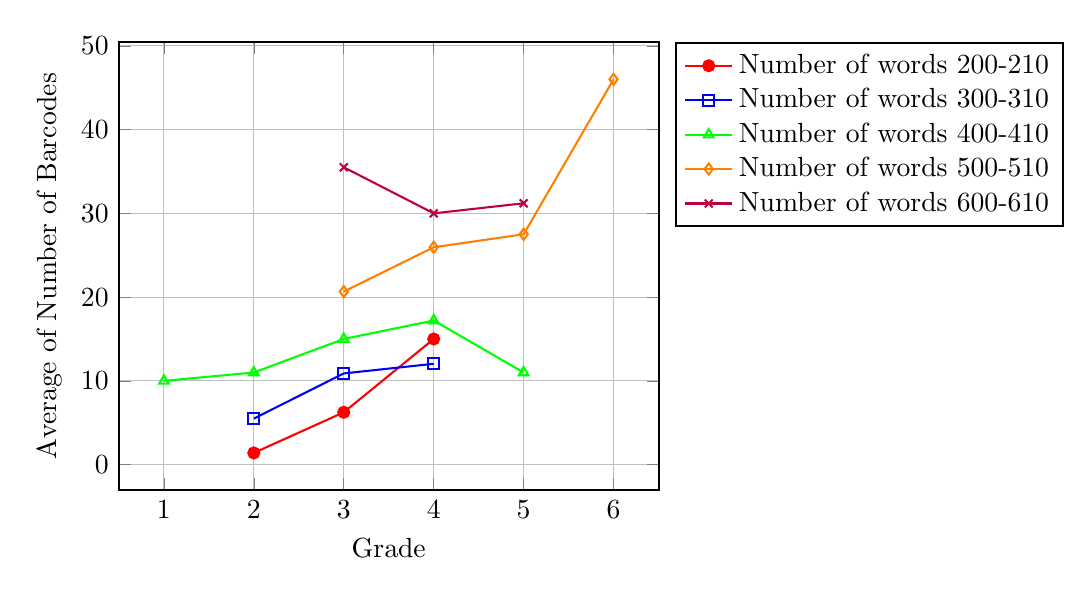
\begin{tikzpicture}
    \begin{axis}[
      xlabel={Grade},
      ylabel={Average of Number of Barcodes},
      legend pos=outer north east,
      grid=both,
    ]
    
    % Number of words 200-210
    \addplot[color=red,mark=*] coordinates {
      (2, 1.4)
      (3, 6.25)
      (4, 15.0)
    };
    
    % Number of words 300-310
    \addplot[color=blue,mark=square] coordinates {
      (2, 5.5)
      (3, 10.89)
      (4, 12.04)
    };
    
    % Number of words 400-410
    \addplot[color=green,mark=triangle] coordinates {
      (1, 10.0)
      (2, 11.0)
      (3, 15.0)
      (4, 17.21)
      (5, 11.0)
    };
    
    % Number of words 500-510
    \addplot[color=orange,mark=diamond] coordinates {
      (3, 20.66)
      (4, 25.95)
      (5, 27.5)
      (6, 46.0)
    };
    
    % Number of words 600-610
    \addplot[color=purple,mark=x] coordinates {
      (3, 35.5)
      (4, 30.0)
      (5, 31.2)
    };
    
    \legend{
      Number of words 200-210,
      Number of words 300-310,
      Number of words 400-410,
      Number of words 500-510,
      Number of words 600-610
    }
    
    \end{axis}
    \end{tikzpicture}

  \caption{Grades and averages of number of holes within fixed sentence/word number ranges}
  \label{tab:gar}
\end{figure}

Seeing Figure~\ref{tab:gar}, we indeed observe and confirm the correlation of increase
that we conjectured. However, the correlation is not absolute as we can constate.
This is because we don't have enough data (for almost all contradictory data
we have selected only one essay of that grade in that range) and other factors than the argument
do affect the grade too (barcodes only show the structure of an essay, for which we
chose to do the tests on discoursive essays). Typically, the wording
of essays of grade 3 but with 30-40 barcodes is bad and repetitive, which is
probably the reason why they are graded not high.

In conclusion, while in Figure~\ref{fig:ads} we have enough essays as example with the default that
the method(division) is not rigorously convincing, and in Figure~\ref{tab:gar} we don't
have enough essays for each range though the method is solid, with them combined,
we are confident that the number of barcodes of dim 1 is a good mesure of the quality of
argument structure of an essay.

\paragraph{Further} We may provision studying the identification of type
of arguments (or in previous case, type of comments) by exploiting persistent homology structure,
trying higher dimensional persistent homology etc. But our journey ends here.

\subsection{Theoretical}
\label{theoretical}

This content is a synthesis of this course\cite{INF556} and other
information on the internet.

\paragraph{Motivation} Given a point set, find the underlying (homological) structures of
the data. First, let's consider a topological space, how do we determine
the homology structure of the space in a computational way.

\begin{definition}[$p$-simplex ($p\in\N$)]
  Let $V$ be some finite set (the vertices).
  A $p$-simplex $\sigma$ is the convex hull of $p+1$
  points $x_0, \ldots, x_p \in V$.
  We denote $\sigma = \conv\{x_0, \ldots, x_p\}$ a subset of $V$.
\end{definition}
\RM In practice, we simplify a topological space to its homology equivalence (thin
triangulation) without
losing the information we want (connected components, holes).

\begin{definition}[Face]
  A face of $\sigma$ is $\conv(S)$ where $S\subset\{x_0,\ldots, x_p\}$
\end{definition}

\begin{definition}[Simplicial complex]
  A simplicial complex $X$ is a finite collection of simplices s.t.
  $$
  \forall \sigma\in X, \forall \tau\subset\sigma, \tau\in X
  $$
\end{definition}

\begin{definition}[Chain space]
  The vectorial space of $k$-chains of a simplicial complex $X$ over a field $\K$ is defined by:
  $$
  C_k(X) := \left\{\sum_{i=1}^{\left|X_k\right|} \alpha_i \sigma_i: \alpha_i \in \mathbb{K}, \sigma_i \in X_k\right\}
  \simeq \K^{|X_k|}
  $$
  where $X_k = \{A\subset X : |A|=k+1\}$ the set of $k$-simplexes in $X$.
\end{definition}
\RM Let's work with $\K = \Z/2\Z$ so that we don't consider orientation.

\begin{definition}[$p$-chain]
  A $p$-chain is a subset of $p$-simplices in a simplicial complex $X$.
\end{definition}

\begin{definition}[Boundary operator]
  $$
  \begin{aligned}
  \partial_k: C_k(X) & \to C_{k-1}(X) \\
  \sigma=\{ v_0, \ldots, v_k \} & \mapsto \sum_{j=0}^k(-1)^j \underbrace{ \{v_0,\ldots,v_k \} \setminus \{v_j\}}_{\in X_{k-1}} \\
  \left(\lambda \sigma+\sigma^{\prime}\right) & \mapsto \lambda \partial_k \sigma+\partial_k \sigma^{\prime} \text{ (linear extension)}
  \end{aligned}
  $$
\end{definition}

\begin{lemma}
  $$
  \forall k, \partial_k \partial_{k+1} = 0
  $$
  \label{lem:pp0}
\end{lemma}

\begin{definition}[$k$-th homology group]
  \begin{itemize}
    \item $k$-cycles : $Z_k:=\Ker(\partial_k)$
    \item $k$-boundaries : $B_k:=\Im(\partial_{k+1})$
  \end{itemize}
  The $k$-th homology group of $X$ for the field $\K$ is the following quotient
  of vector spaces:
  $$
  H_k(X):={Z_k\over B_k}
  $$
  (well defined because of the Lemma~\ref{lem:pp0})
  The $k$-th Betti number $\beta_k = \mathrm{rank}(H_k)$.
\end{definition}
\RM The computational method is by Gauss elimination, we omit it here
because we later introduce a method to calculate barcodes which is more
powerful and uses Gauss elimination too.

Now, we are able to give the homology structure of a given topological space (simplicial complex).
Let's go back to the beginning, initially, we are only given a point set,
we may link the points in the set to form a simplicial complex.
The way in which we link the points change our view of the underlying structure.
The scale matters Figure~\ref{fig:scale}.


\begin{definition}[Filtration]
  A filtration over $T$ is a family $\F = (F_t)_{t\in T}$ of increasing topological spaces:
  $$
  \forall t, t^{\prime} \in T, t \leqslant t^{\prime} \Rightarrow F_t \subset F_{t^{\prime}}
  $$
\end{definition}

\begin{definition}[Persistence module]
  Let $\mathbb{K}$ be a given field. A persistence module over $T \subset \mathbb{R}$ is a family $\mathbb{V}=\left(V_t\right)_{t \in T}$ of $\mathbb{K}$-vector spaces
  endowed with linear application $v_t^{t^{\prime}}: V_t \rightarrow V_{t^{\prime}}$ induced by
  a filtration by being applied $H_k$ (e.g.\ Figure~\ref{fig:tda_diagram}).

  $\I_{[l, r)}$(or $\I_{[l, r]}$ etc.) is an interval module with $T = [l, r)$,
  $(V_t)_t = (\K)_t$, $(v^{t'}_t) = (\id)$.
\end{definition}

\begin{theorem}[Decomposition theorem]
  A persistence module $\mathbb{V}$ can be decomposed as a direct sum of interval module
  in the following case (sufficient, not necessary):
  \begin{itemize}
    \item If $T$ is finite. [Gabriel, 72]
    \item When all the vector spaces $V_t$ are finite-dimensional. [Crowley-Boevey, 2012]
  \end{itemize}
  Furthermore, when it exists, the decomposition is unique (up to isomorphism and ordering of terms).
  See an example at Figure~\ref{fig:tda_diagram}
\end{theorem}

\RM Intuitively, the way to decompose is beginning from where a cycle occurs
and following the linear map until it diminishes and concluding an interval module;
the multiset of pairs of extremities of the intervals obtained by decomposition is called the \textbf{barcodes}
or the persistence diagram; to compute the decomposition, we do Gauss elimination (explained in the following).

\subsubsection{Algorithm to calculate the persistence diagram}

\paragraph{Input} A simplicial filtration, that is a filtration over a simplicial complex $K$ which verifies:
\begin{itemize}
  \item $T=\{1, \ldots, m\}$ (finite, so we have a decomposable filtration).
  \item $K_1=\{\sigma_1\}, K_m = K$
  \item $\forall t \in T, K_t$ is a simplicial complex,
  which is a sub-complex of $K_{t+1}$.
  \item We only add one simplex at each step,
  that is $K_{t+1} \backslash K_t=$ $\left\{\sigma_{t+1}\right\}$.
\end{itemize}

\begin{algorithm}
  \caption{Compute the barcodes corresponding to a simplicial filtration}
  \begin{algorithmic}
  \State M := the matrix of boundray operator $\partial$ =: $(c_0, \ldots, c_m)$
  \State $\mathrm{low}(j):=\left\{\begin{array}{l}\max \left\{i \mid M_{i j} \neq 0\right\} \\ 0 \text { if } M_{i j}=0 \text { for all } i\end{array}\right.$
  \For{$j = 1\ldots m$}
  \While{$\exists i<j$ s.t. $\mathrm{low}(i)=\mathrm{low}(j) \neq 0$}
  \State $c_j \gets c_j+c_i$ (Still working with $\K = \Z/2\Z$)
  \EndWhile
  \EndFor
  \State Barcodes are $\{(i, \max\{j \mid \mathrm{low}(j)=i\}) \mid c_i = 0\}$
  (1. This is a multiset 2. $\max$ return $\infty$ if empty 3. the set where we take max is of size at most 1)
  \end{algorithmic}
\end{algorithm}

\begin{proof}[Proof of validity]
Each $c_i = 0$ means the birth of a cycle (one plus for the dimension of the kernel).
Each $c_i \not= 0$ trivialize a cycle (one plus for the dimension of the image).
It remains to show that the pairing is right.

Consider a $c_j \not= 0$, $c_j = e_{l_1} + \cdots + e_{l_k}~(0\le l_1 < \cdots < l_k < j)$.
Note that $\partial_d (\sigma_{l_1} + \cdots + \sigma_{l_k}) = 0$ (Lemma~\ref{lem:pp0}).
So $c_{l_k} = 0$. A posteriori, we can say that $(\sigma_{l_1} + \cdots + \sigma_{l_k})$
this cycle is created at $l_k$ as in a base of $\Ker \partial_d$ (we construct
such base a posteriori in this way).

So the pairing is right.

\end{proof}

\subsubsection{Stability theorem}

\newcommand{\Dg}{\mathrm{Dg}}

\begin{definition}[Homological critical value]
  Let $X$ be a topological space and $f : X \to \R$ a function.
  A homological critical value of $f$ is a real number $b$ for which
  there exists an integer $k$ such that $\forall \epsilon > 0, $
  $H_k(f^{-1}(-\infty, b-\epsilon]) \to H_k(f^{-1}(-\infty, b])$ is not
  an isomorphism.
\end{definition}

\begin{definition}[Tame]
  A function $f : X \to \R$ is tame if it has a finite number of homological
  critical values and the homological groups $H_k(f^{-1}(-\infty, a])$ are finite-dimensional
  for all $k\in\Z$ and $a\in\R$.
\end{definition}
\RM So that the first condition of the decomposition theorem is satisfied
and we have a finite number of barcodes.

\begin{theorem}[Stability Theorem]
  For any two tame functions $f, g : X \to \R$
  $$
  d_\infty(\Dg~f, \Dg~g) \le \|f-g\|_\infty
  $$
  where
  $$
  d_\infty(\Dg~f, \Dg~g) =
  \inf_{m : \Dg(f)\sqcup \Delta \stackrel{\sim}{\to} \Dg(g)\sqcup \Delta}
  ~~
  \sup_{t\in \Dg(f)\sqcup \Delta} \|t-m(t)\|_\infty
  $$
  and $\Dg$ denotes the persistence diagram.
\end{theorem}

\begin{figure}
\centering
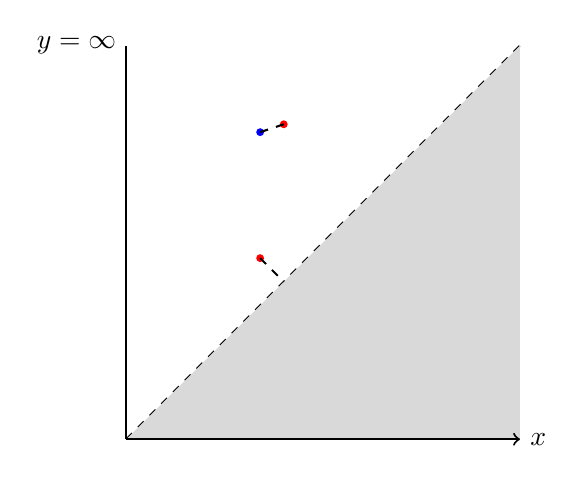
\begin{tikzpicture}
  \draw[dashed] (0, 0) -- (5, 5);
  \fill[gray!30] (0, 0) -- (5, 5) -- (5, 0) -- cycle;
  \draw[->] (0, 0) -- (5, 0) node[right] {$x$};
  \draw[-] (0, 0) -- (0, 5) node[left] {$y=\infty$};
  \fill[red] (1.7, 2.3) circle (0.05);
  \fill[red] (2, 4) circle (0.05);
  \fill[blue] (1.7, 3.9) circle (0.05);

  \draw[dashed] (2, 4) -- (1.7, 3.9);
  \draw[dashed] (1.7, 2.3) -- (2, 2);
\end{tikzpicture}
\caption{Barcodes matching on a persistence diagram}
\label{fig:persistence diagram domaine}
\end{figure}

\begin{proof}
  Let $f, g : X \to \R$ be 2 tame functions. We denote $\varepsilon = \|f-g\|_\infty$.
  We pose $F_t = f^{-1}((-\infty, t]), G_t = g^{-1}((-\infty, t])~(t\in \R)$.

  Key observation: $\left\{F_t\right\}_{t \in \mathbb{R}}$ and $\left\{G_t\right\}_{t \in \mathbb{R}}$
  are $\varepsilon$-interleaved w.r.t. inclusion:\\
  $$
  \forall t \in \mathbb{R}, G_{t-\varepsilon} \subseteq F_t \subseteq G_{t+\varepsilon}
  $$

  We denote
  $F^{2 \varepsilon}=\left\{F_{2 n \varepsilon}\right\}_{n \in \mathbb{Z}}$,
  $G^{2 \varepsilon}=\left\{G_{2(n+1) \varepsilon}\right\}_{n \in \mathbb{Z}}$
  2 discret filtrations.
  $$
  \cdots \subseteq F_0 \subseteq G_{\varepsilon} \subseteq F_{2 \varepsilon} \subseteq \cdots \subseteq G_{(2 n-1) \varepsilon} \subseteq F_{2 n \varepsilon} \subseteq G_{(2 n+1) \varepsilon} \subseteq \cdots
  $$
  We denote another discret filtration $\left\{H_{n \varepsilon}\right\}_{n \in \mathbb{Z}}$, where $H_{n \varepsilon}=\left\{\begin{array}{l}F_{n \varepsilon} \text { if } n \text { is even } \\ G_{n \varepsilon} \text { if } n \text { is odd }\end{array}\right.$

  $$
  d_\infty(f, g) \le d_\infty(f, F) + d_\infty(F, H) + d_\infty(H, G) + d_\infty(G, g)
  \le (2+1+1+2)\varepsilon \le 6\varepsilon
  $$
  (We can optimise it to $\varepsilon$)
  
\end{proof}
